\chapter{Introduction}
\section{Motivation}

\section{Objectives}

\chapter{Fundamentals}
\section{ROS}
\section{MCA}
\section{Kinect}
\section{Laser Scanner}
3D laser scanner use narrow laser-beam to scan their environment and allow almost continuous scanning - regardless of whether objects are moving or not. As a result, 3D laser scanner gets a set of points which represent the direction and distance of objects in around. Sick LMS100 (shown in Figure \ref{Laser}) has the scanning angle of  270$^\circ$ and has high detection capability.

We can get the output from laser scanner in ROS with sensor\_masgs/LaserScan message. The message is made up of several parts, including header, ranges, and other information of laser scaner. The start and end angle of the scan, angular distance between measurements, time between measurements, minimum and minimum range value are stored in this message. Most important information we need is the angle of each hit and its distance (range) from the scanner.

\begin{figure}[thpb]
      \centering
      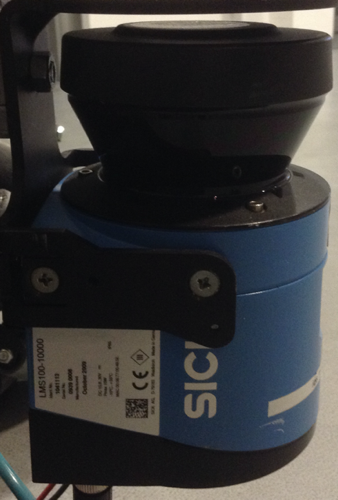
\includegraphics[width=0.5\textwidth]{graphics/Laserscanner.png}
      %\includegraphics[scale=1.0]{figurefile}
      \caption{Sick LMS100}
      \label{Laser}
   \end{figure}
\section{ASAP (Advanced Shared Autonomy Platform)}
<<<<<<< HEAD
The ASAP (shown in Figure \ref{ASAP}), short for Advanced Shared Autonomy Platform, is a mobile robotic platform based on two Segway RMP-50 Omni platforms. The Platform is mounted with four omnidirectional plastic rollers, so that the Segway can free move in all directions (shown in Figure \ref{Omni}). In addition, this ASAP includes some sensors, on-board comoputer, software system. For sensor, there are Two Sick LMS100 laser scanners and a Kinect on top. The embeded computer is Esperia, which has 4G ram, 64G SSD, core i7 M620 CPU and can be connected through WLAN address 141.21.13.215. Ubuntu 14.04 Trusty, ROS Indigo, MCA2 are three main software systems in this ASAP.

\begin{figure}[thpb]
      \centering
      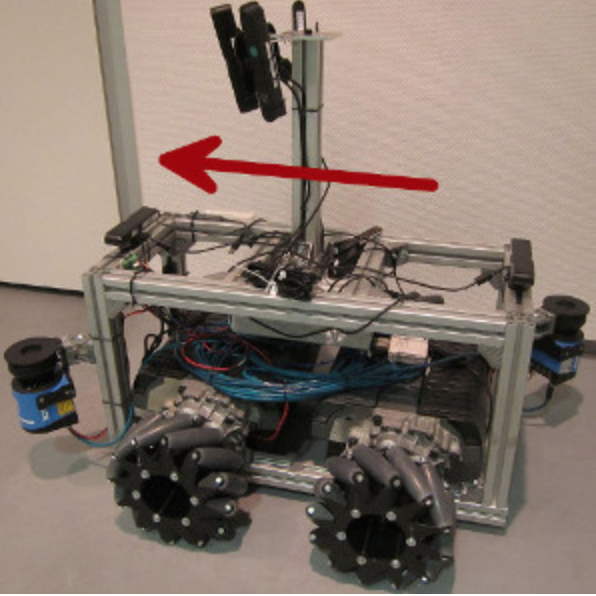
\includegraphics[width=0.5\textwidth]{graphics/ASAP.png}
      %\includegraphics[scale=1.0]{figurefile}
      \caption{The structer of Advanced Shared Autonomy Platform, and red arrow shows the forward direction of the platform, which is the same as the X axes in ROS.}
      \label{ASAP}
   \end{figure}

\begin{figure}[thpb]
      \centering
      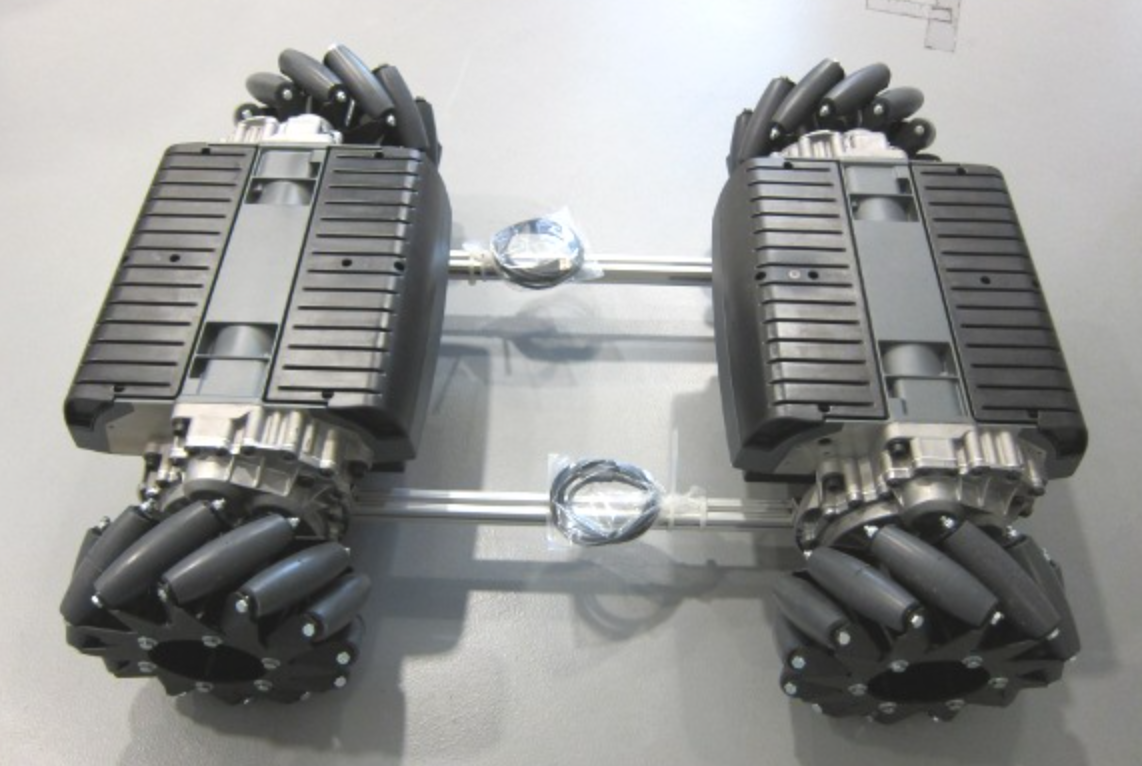
\includegraphics[width=0.5\textwidth]{graphics/SegwayPlattform.png}
      %\includegraphics[scale=1.0]{figurefile}
      \caption{The Segway RMP-50 Omni Plattform includes Mecanum-Rad and Batterie.}
      \label{Omni}
   \end{figure}
=======

\section{Kalman Filter}
Many problems in the domain of artificial intelligence require the prediction of future states by evaluating measurements. Around the 1960s Peter Swerling, Rudolf E. Kálmán, Thorvald N. Thiele and Richard Bucy described an algorithm for this purpose. It is now known as the \textit{Kalman filter}.

In the field of robotics Kalman filters can be utilized to predict future poses for a moving robot by continuously combining measurements from various sources. A Kalman filter is therefore a sensor fusion algorithm. Common sensors are
 
\begin{itemize}
\item motion sensors that estimate position change over time (odometry),
\item laser scanners that scan the environment,
\item cameras that track predefined markers. 
\end{itemize}

By combining the last estimation and the current sensor outputs a new estimation for the current state is obtained. In this process two steps are commonly distinguished: \textit{predict (a priori)} and \textit{update (a posteriori)}.
\\\\
During \textbf{prediction} the next state as well as its covariance are estimated. After that new sensor data is compared with the predicted state, which results in the calculation of the so-called  Gain. The Kalman Gain is an indicator for the certainty of both measurements and prediction. High covariances in the prediction increase the Gain while high covariances in the measurements decrease it.

$$\text{a priori state estimate:} $$
$$\text{a priori covariance estimate:} $$

This will result in the filter trusting either the measurements or the predictions more depending on the gain. 
\\\\
Based on the Gain the Kalman filter produces a posteriori state and covariance estimates during \textbf{update phase}. The higher the gain, the closer these estimates will be to the measurement output and vice versa.

$$\text{a posteriori state estimate:} $$
$$\text{a posteriori covariance estimate:} $$
>>>>>>> 64297137279947590838a6c0f7705ab555d30708
